\textbf{Прим.} Билет взят из открытых источников: \href{https://towardsdatascience.com/understanding-the-bias-variance-tradeoff-165e6942b229}{1} \href{https://en.wikipedia.org/wiki/Bias%E2%80%93variance_tradeoff#:~:text=The%20bias%E2%80%93variance%20decomposition%20is,noise%20in%20the%20problem%20itself.}{2} (тема не найдена на лекциях)
\\

Цель билета - рассказать о проблеме поиска балланс между недообучением и переобучением.

\textit{Компромисс между смещением и дисперсией} - это свойство набора моделей предсказания, когда модели с меньшим отклонением (low bias) от имеющихся данных имеют более высокую дисперсию (high variance) на новых данных (то есть подвержены переобучению), и наоборот модели с меньшей дисперсией (low variance) от имеющихся данных имеют более высокое смещение (high bias) на новых данных (это приводит к недообучению). Ниже более подробное объяснение этого процесса. Возникает конфликт при попытке одновременно минимизировать эти два источника ошибок, которые мешают алгоритмам обучения с учителем делать обобщение за пределами тренировочного набора.

Смещение - это разница между средним прогнозом нашей модели и правильным значением, которое мы пытаемся предсказать. Модель с высоким смещением уделяет очень мало внимания данным обучения и чрезмерно упрощает модель. Это всегда приводит к высокой погрешности в обучающих и тестовых данных. (недообучение).

Дисперсия - это изменчивость прогноза модели для данной точки данных или значения, которое говорит нам о разбросе наших данных. Модель с высокой дисперсией уделяет большое внимание обучающим данным и не обобщается на данные, которые она раньше не видела. В результате такие модели очень хорошо работают с обучающими данными, но имеют высокую частоту ошибок в тестовых данных. (переобучение)
\\
\textbf{Математическое обоснование}

Пусть переменная, которую мы пытаемся предсказать, равна $Y$, а другие ковариаты - $X$. Мы предполагаем, что между ними существует такая взаимосвязь, что
$Y=f(X) + e$. Где $e$ - член ошибки, и он обычно имеет матожидание 0.

Мы создадим модель $\hat{f}(X)$, используя линейную регрессию или любой другой метод моделирования.
Таким образом, ожидаемая квадратическая ошибка в точке $x$ равна

$$Err(x) = \mathbb{E}[(Y - \hat{f}(x))^2]$$

Можно разложить в:

$$Err(x) = (\mathbb{E}[\hat{f}(x)] - f(x))^2 + \mathbb{E}[(\hat{f}(x) - \mathbb{E}[\hat{f}(x)])^2] + \sigma^2_{e}$$
$$Err(x) = Bias^2 + Variance + Irreducible Error$$

$Err(x)$ - это сумма смещения$^2$, дисперсии и неустранимой ошибки.

Неустранимая ошибка - это ошибка, которую нельзя уменьшить путем создания хороших моделей. Это показатель количества шума в наших данных.

\begin{figure}[h]
\centering
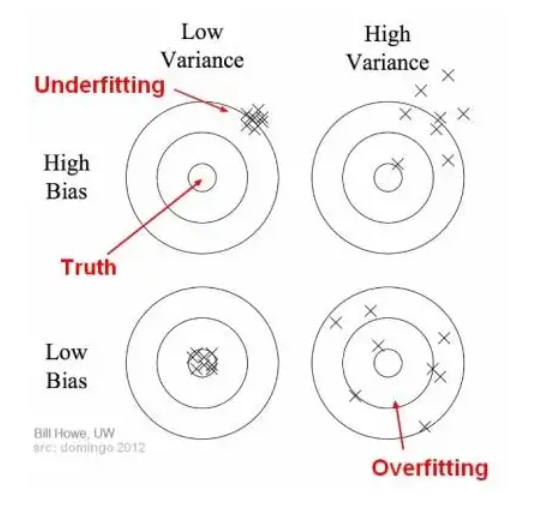
\includegraphics[width=0.4\linewidth]{15.1.PNG}
\caption{Расположение тестовой выборки относительно модели.}
\end{figure}
\\
\textbf{Проблема Bias-Variance Tradeoff}

Это проблема сравнения $Bias^2$ vs. $Variance$. Если наша модель слишком проста и имеет очень мало параметров, она всего будет иметь большое смещение и низкую дисперсию. С другой стороны, если наша модель имеет большое количество параметров, она будет иметь высокую дисперсию и низкое смещение. Поэтому нам нужно найти правильный/хороший баланс без переобучения и недообучения данных. Для этого, нам нужно найти хороший баланс между смещением и дисперсией таким образом, чтобы свести к минимуму общую ошибку.

$$TotalError = Bias^2 + Variance + Irreducible Error$$

\begin{figure}[H]
\centering
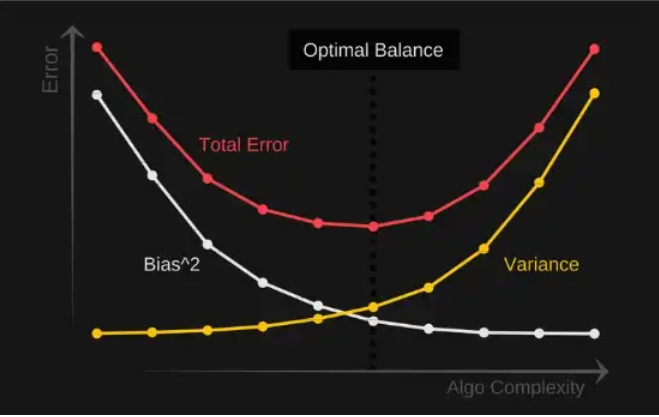
\includegraphics[width=0.4\linewidth]{15.2.PNG}
\caption{}
\end{figure}